\documentclass[12pt]{report}
\usepackage{tikz}
\usepackage{cite}
\usepackage{listings}
\usepackage{url}
\RequirePackage{graphicx}
\graphicspath{ {images/} }
\newcommand{\ppt}{\textbf{p.p.t.}}
\newtheorem{theorem}{Theorem}[section]
\newcommand{\GF}{\text{GF}}
\newcommand{\xor}{\oplus}
\theoremstyle{definition}
\newtheorem{definition}{Def.}

\renewcommand{\collaborators}{Jiachun Zhang}

\begin{document}

\maketitle

\setcounter{MaxMatrixCols}{20} \setlength\parindent{0pt}

\section{Introduction}
The hearing of a music can be seen as a complex procedure of recognition. 
When we hear a music, we can recognize the genre, characteristic, and 
style traits of its composer. Sometimes, we can immediately recognize
the similarity between two pieces of music, be it the reference from one to another
, same chord relation, or a signature musical device being used. In this project, 
we will make an attempt to examine the similarity between two pieces of music using 
various metrics ranging from the cosine similarity to DFT. The project will
survey on the existing methods of music similarity proposed by music theorists
Dimitri Tymoczko, David Lewin, and Jason Yust. As a related topic, the project has also
investigated the key-finding algorithm orginally proposed by Krumhansl and Schmuckler, 
modified by David Temperley. The final section of the report will be questions raised 
in the progress of reviewing these works and implementing the algorithms.

\section{Cosine Similarity}
In the context of atonal music, because how the music is composed, we shall use a 
deterministic method to find the similarity between two set of pitch classes by looking 
at the prime form of them. However, in the context tonal music, there is no such 
structure to describe this abtract concept of a original form easily. But even without 
rigorous hearing training or abundant listening experience, one can identify the
musical devices used in a piece of music easily. For example, a perosn
without any knowledge in music theory should have no problem to identify 
a phrase was transposed to a different key or the exact same motif being 
repeated over and over again. In such sence, we shall apply cosine similarity 
on two set of scale degrees in an interval vector.
\paragraph*{Application}
    Let us first look at a simple operation in tonal music -- Transposition. Transpositon moves a 
collection of notes by certain interval. It is very common in classical music the opening
statement is transposed to the dominant key. We shall
write a very simple melody in the key of C:

\begin{center}
    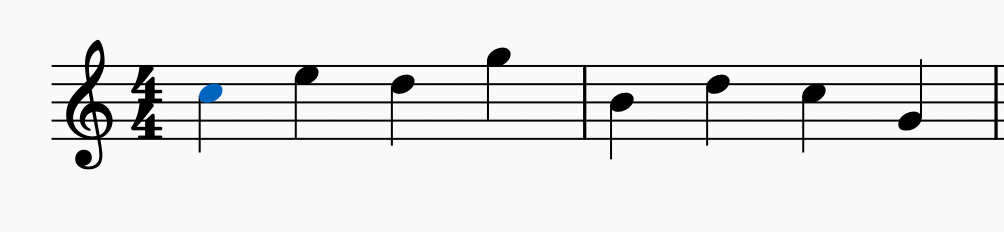
\includegraphics{1}
\end{center}

We can write these notes in a vector form $[0, 4, 2, 7, 11, 2, 0, 7]$. The phrase
starts with C and ends in G. Transpose it strickly to its dominant key, G, we get:
\begin{center}
    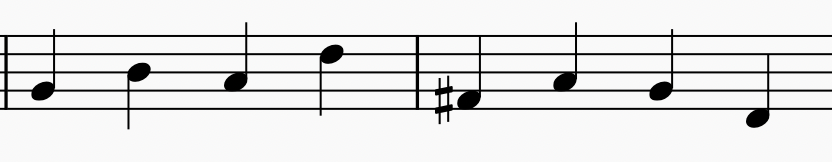
\includegraphics{2}
\end{center}
The second phrase is now in the key of G. We can write it in vector 
form $[7, 11, 9, 2, 6, 9, 7, 2]$. We know it is an element in the T7 group,
which transpose everything up by 7 or down by 5 semitones. But sometimes 
the phrase can be twicked a little bit to make it more interesting. For example,
the second phrase can be written as follows:
\begin{center}
    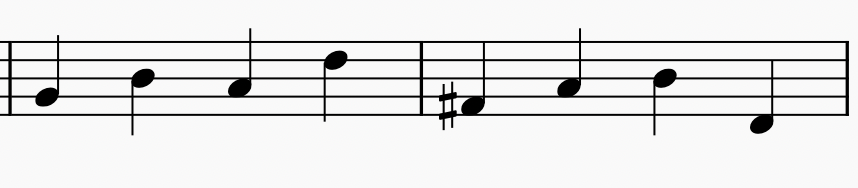
\includegraphics{3}
\end{center}
G in the second bar now becomes B, are they still similar in some way? 
We as humans can tell they are similar by ear easily, but how can we show they are 
similar by numbers? One possible way we can do is to calculate their "cosine similarity". 
We shall calculate differences between first and 2 other phrases, whcih can written as $u, v$:
\[[7,7,7,7,7,7,7,7], [7,7,7,7,7,7,11,7]\] and then calculate the cosine similarity between them:
$\cos(u, v) = \frac{u\cdot v}{|u|\cdot |v|}\approx0.98$.\\
This is just one method of looking at melodic similarity, which might be not acurate since
it does not consider the potential harmoic information implied by the melody, or base 
accompanied. Nevertheless, we can see a simple analysis used in the interval space
can two sets of pitch classes are related.

\section{Key Finding Algorithm}
Key and scale degree is a special concept in tonal music. When comparing 
similarity between two tonal pieces, knowing what key they are in gives us
very crucial information. The current popular key-finding algorithm is
proposed by Krumhansl and Schmuckler, which is based on the idea of
"the most prominent note". However, Temperly points out some flaws in this
algorithm, and proposes a modified version of it. 
\begin{enumerate}
    \item The defects of the original Krumhansl and Schmuckler:
    \begin{enumerate}
        \item The notes are "weighted" by duration, which means repeated notes would take on more weight which might alter the final decision.(P196)
        \item It does not take into the account of modulation between different keys.(P198)
        \item The original key-profile model did not distinguish between different spelling fo the same pitch (A#=Gb).(P199)
    \end{enumerate}
    \item The solution to the problems above:
    \begin{enumerate}
        \item Binary representation { 0, 1 } given certain metrical unit(mesure, second, etc) in terms of prescence.
        \item Calculate a key for segmented phrases. Introduce "change penalty" ig the key for one segment differs from the key of the previous segment until the score for new key is the dominant key.
        \item Infer the speeling might be "cheating" in some sense, so not addressed.
    \end{enumerate}
\end{enumerate}

\paragraph*{Baysian Modeling}
We can see music as the duality of structure and surface.
Recover the multiple possible strcutures (keys) from a single representation of the surface (notes). And we want to select the best one:
\[\arg\max_{\text{structure}}\Pr[\text{structure}|\text{surface}]\]
Using Bayes' rule, We have:
\[\Pr[\text{structure}|\text{surface}]=\frac{\Pr[\text{surface}|\text{structure}]\Pr[\text{structure}]}{\Pr[\text{surface}]}\]
Since for any structure, $\Pr[\text{surface}]$ stays the same, 
we only need to consider \\$\arg\max_{\text{structure}}\Pr[\text{surface}|\text{structure}]\Pr[\text{structure}]$.
But, The Krumhansl-Schmuckler was tested on Bartok's \emph{14 Bagatelles Op.47 No.1}. The
algorithm regonized the right hand part as in E major/C\# minor, but ignored
the entire left hand in C Locrian/G Lydian. This is expected, since
the algorithm only outputs one key given all notes in the piece and 
it seems like notes in the left hand sums up to a less duration than
the right hand. So the KS algorithm put more weights in right hand than the
left. 
\section*{Set-Class similarity and Fourier Transform}
Fourier transform assign two-dimensional vector whose components are:
\[V_{p,n}=(\cos(2\pi pn/12), \sin(2\pi pn/12))\]
Where for integer $n$ from $0$ to $6$ and $p$ in $\{0...11\}$ is the pitches
in a chord. Each fourier component is the sum of all such component:
\[n\text{th Fourier Component}=\sum_{p\in v}V_{p,n}\]
\begin{itemize}
    \item Voice leading and set-class similarity. Steps
    to find the minimal Euclidean voice leading between two n-note 
    multiset-classes $A$ and $B$:
        \begin{itemize}
            \item Choose a representative (prime form?) of $A$ calculate 
            the sum of its pitch classes.
            \item Find the $n$ (12/n semitones for each) 
            transpositions of $B$ with the same sum.
            \item For each of the transposition, calculate the $L_2$
            norm of $A$ and the vector. Do the same for inversions.
            \item Take the minimum of these $2n^2$ numbers and output the 
            result.
        \end{itemize}
    \item Fourier Magnitude
        \begin{itemize}
            \item In a set class space constructed by pitches of some 
            perfectly even $n$-note chord, $n\in\{1...6\}$. Note the $n$-note
            chord means the chord even seperate the $12$ tone equal 
            temperament pitches. 
            \item Given a $x$-note set-class space, the $n$th Fourier component of a chord will decrease 
            as pitches move away from the subset of pitches in $n$ notes 
            chord. Illustrated below:
            \begin{figure}[h]
                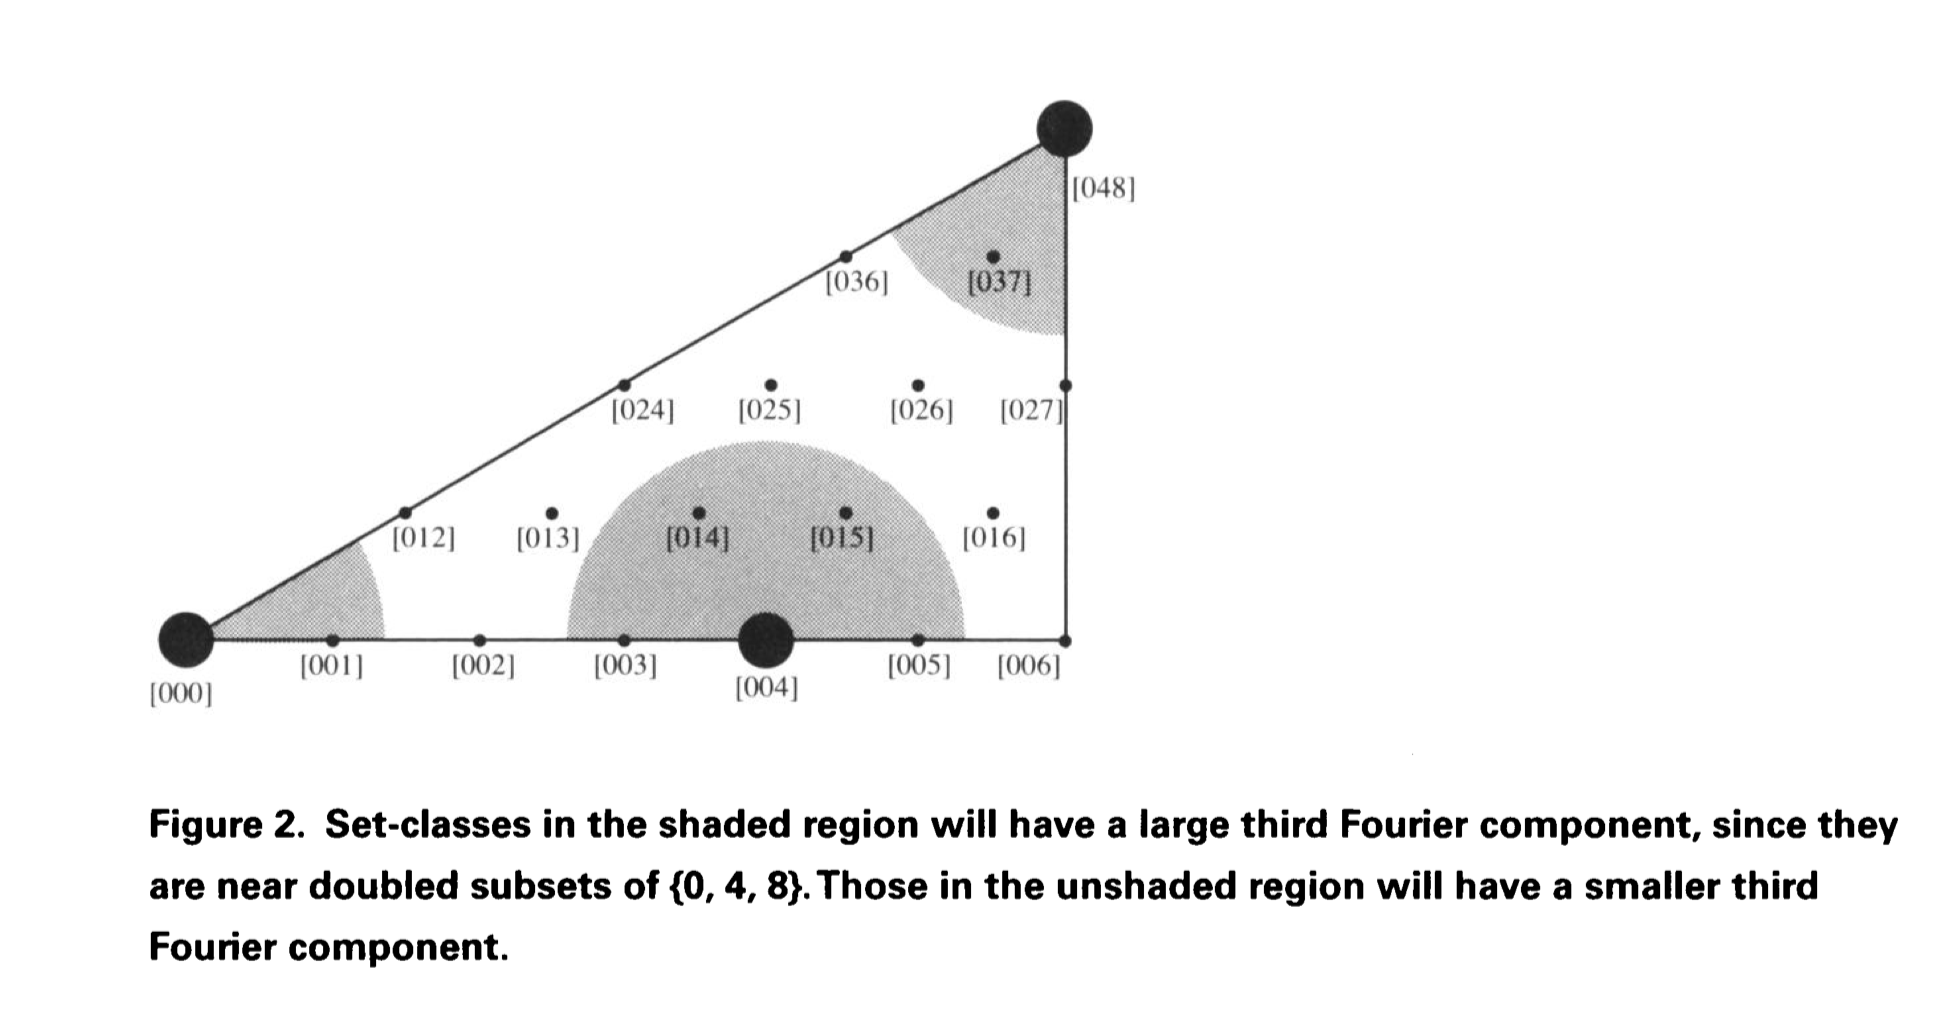
\includegraphics[scale=0.5]{Tymoczko_1.png}
            \end{figure}
            \item We can use a linear equation to estimate the $n$-th
            Fourier component of chord given the \emph{minimal voice leading
            } to the nearest doubled subset(VL). This means there is a 
            close relationship between FC and the minimal Euclidean distance 
            between two chords.
            \item 2 analysis procedure below:
            \begin{figure}[h]
                \centering
                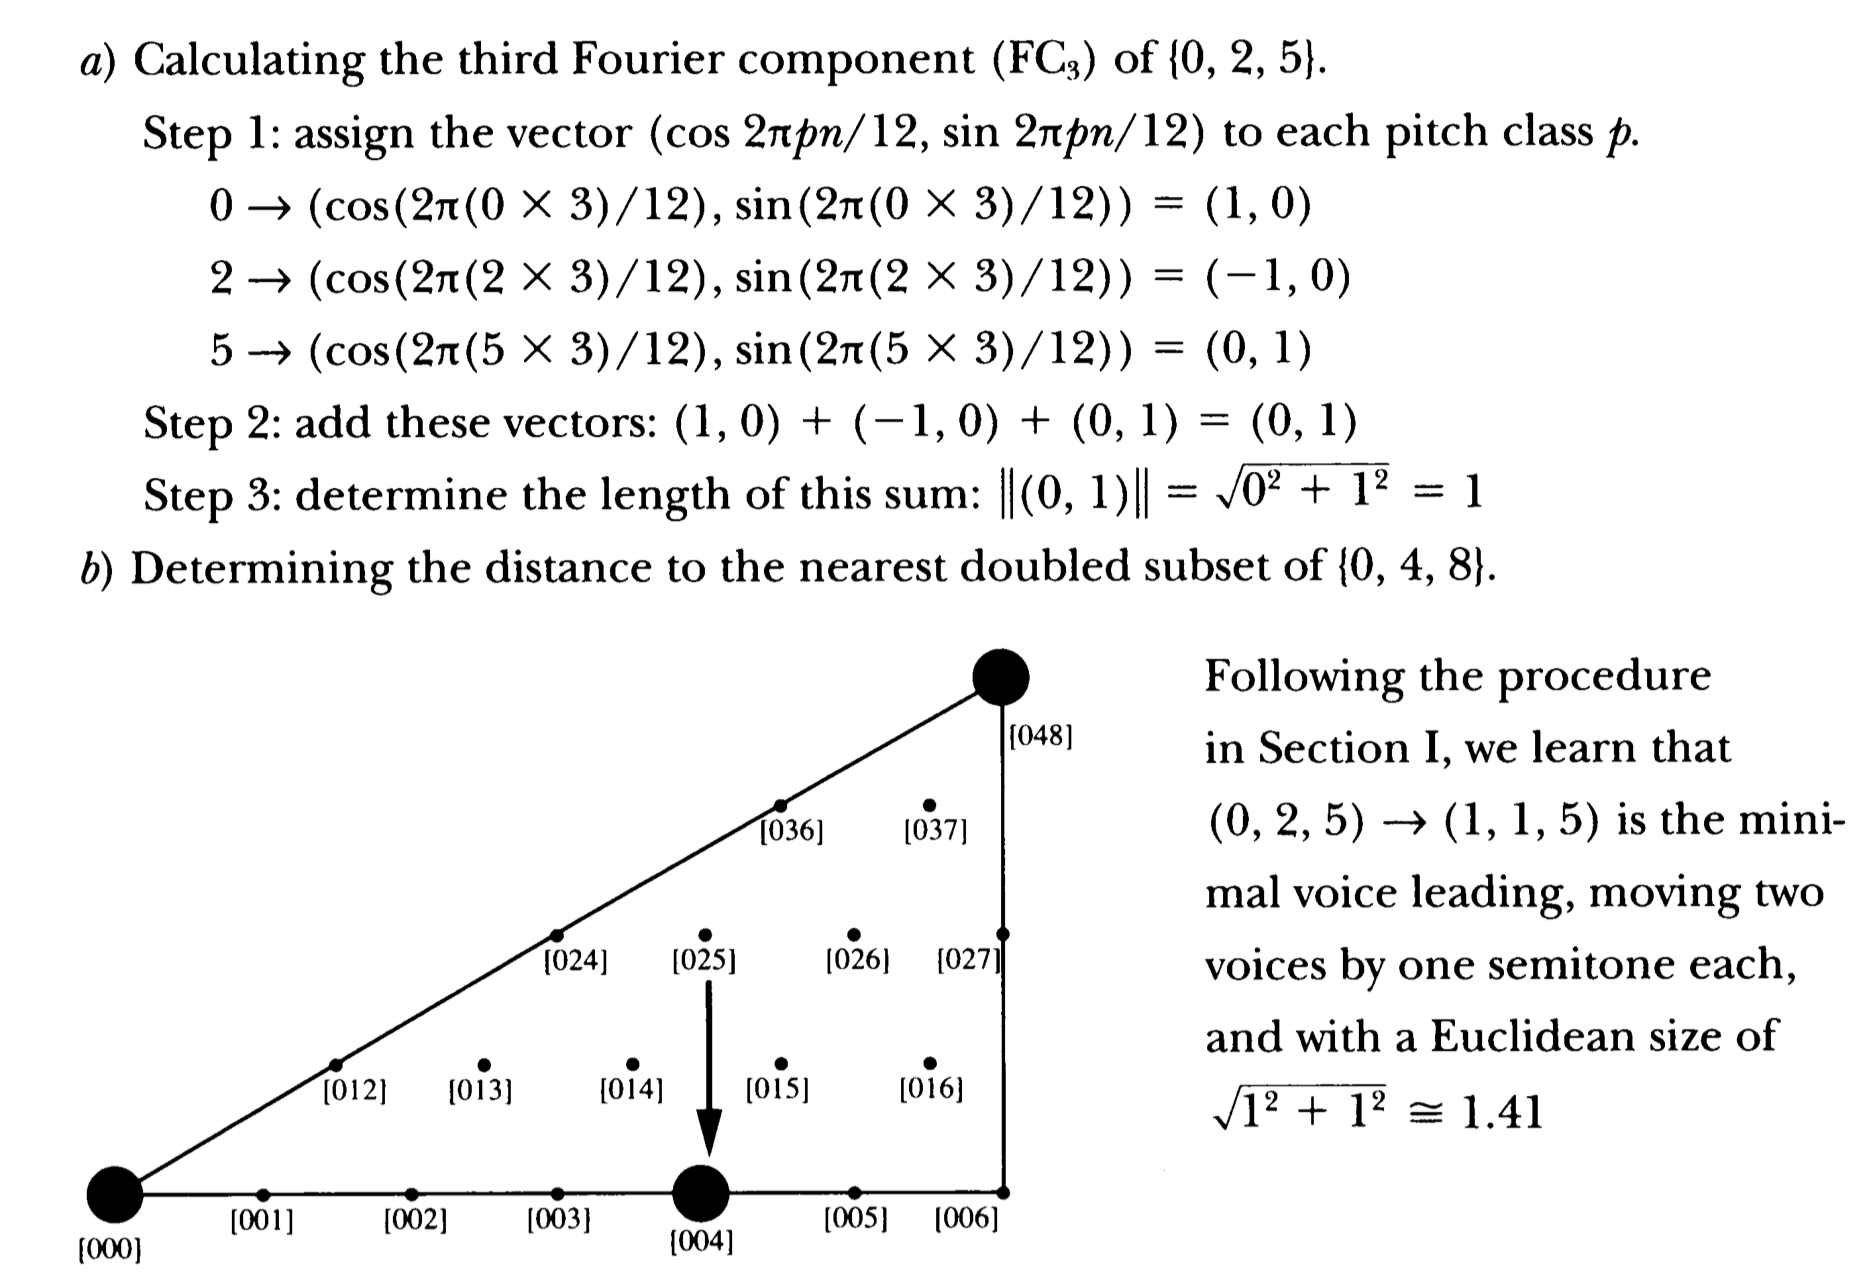
\includegraphics[scale=0.5]{Tymoczko_2.png}
            \end{figure}
            \item The analogy of minimal voice leading on 
            a pitch class circle is: as the Fourier Component increases
            (which is the sum of all vectors), the minal voice leading decreases.
            \item FC6 is the difference absolute value of difference between 
            the number of a chord's notes in one whole tone scale and the nuber 
            of its notes in the other ($[0,2,4,6,8,10],[1,3,5,7,9,11]$).
        \end{itemize}
\end{itemize}
\section{Yust's Set Theory}
Introduced Fourier componenets and phase spaces. 
\begin{itemize}
    \item \textbf{n Phase Space}: A circle evenly divided by $n$ interval(in the context of 12-equal temperament).
    \item \textbf{Fourier Component}: See summarization for Tymoczko's paper.
\end{itemize}
The process is similar to DFT, which can be seen as a matrix multiplication written as:
\[F_k=\frac{1}{n}\sum_{j=0}^{n-1}e^{-2\pi i\frac{jk}{n}}\]
Where $F_n$ is the $n$-th Fourier component, $k$ is the pitch class, and $n=12$. Or, more generally:
$\hat{f_k}=[[\mathsf{DFT}]]\cdot f_k$. Think of the process as matrix multiplication.
Different phase space reveals different properties of music. $Ph_5$ indicates 
the a set's affinity toward diatonic collection. Each $6$ phase space approximates:
\begin{enumerate}
    \item chromaticism
    \item quartal harmony?(not sure what this means)
    \item hexatonicity
    \item octatonicity
    \item diatonicity
    \item whole-tone quality.
\end{enumerate}
\emph{Scale Theory? Eveness? Might need more explanation.}
We can also use DFT to calculate the common tones of two sets. 
\[\frac{1}{12}\sum_{n=0}^{11}|f_n(A)||f_n(B)|cos(\phi_n(A)-\phi_n(B))\].Intuitively,
common tones will show harmonic closeness. Another aspect in the common tone analysis
is the "wormhole" effect. Which is simply apply analysis in two phase spaces.
\section{Conclusion}
The report briefly introduced four methods in finding the music similarity using
\begin{itemize}
    \item Cosine Similarity
    \item Discrete Foruier Transform
    \item n-th Fourier Component analysis.
\end{itemize}
In addition, we also talked about the Krumhansl-Schmuckler algorithm and its
its limitations. What has yet to be discovered is the properties of the DFT matrix
itself. Thus the next step would be decribing musical meaning of things like
eigenvalues and its corresponding eigenvectors.
\begin{thebibliography}{9}

\bibitem{Temperley}
Temperley, David. "A Bayesian Approach to Key-Finding." In Music and Artificial Intelligence, edited by Christina Anagnostopoulou, Miguel Ferrand, and Alan Smaill, 195–206. Lecture Notes in Computer Science. Berlin, Heidelberg: Springer, 2002.
\bibitem{Tymoczko}
Tymoczko, Dmitri. "Set-Class Similarity, Voice Leading, and the Fourier Transform." Journal of Music Theory 52, no. 2 (2008): 251–72.


\end{thebibliography}
\end{document}
